\documentclass[11pt]{article}
\usepackage[margin=1.05in]{geometry}
\usepackage{amsmath,amssymb,amsthm}
\usepackage{booktabs}
\usepackage{tikz}
\usepackage{algorithm}
\usepackage{algpseudocode}
\usepackage[colorlinks=true,linkcolor=blue,citecolor=blue,urlcolor=blue]{hyperref}

\newtheorem{lemma}{Lemma}
\newtheorem{theorem}{Theorem}
\newtheorem{remark}{Remark}

\newcommand{\voles}{\texttt{voles}}
\newcommand{\dd}{\,\mathrm{d}}
\newcommand{\vtwo}{\nu_2}

\title{Fast uniform-mesh Volterra solvers in \voles:\\
the algorithm, its provenance, and its verification}
\author{Notes accompanying the \texttt{fast-uniform-mesh} branch\\
(commits \texttt{782fb58}, \texttt{382ec8d}, \texttt{a56349d})}
\date{July 2026}

\begin{document}
\maketitle

\begin{abstract}
\noindent
These notes document two performance optimizations to the \voles{}
collocation solvers for Volterra equations, in enough detail that a
mathematically literate reader can reproduce them without consulting
other literature or the code. Both exploit the same structural fact: on a
uniform mesh with a convolution kernel $K(t-s)$, every quantity the
solvers precompute depends on a pair of mesh intervals only through their
\emph{lag}. The centerpiece (Sections~\ref{sec:algorithm}--\ref{sec:apply})
is a self-contained account of the blocked-FFT algorithm of Hairer,
Lubich and Schlichte for accumulating Volterra ``history'' sums in
$O(Q\log^2 Q)$ operations instead of $O(Q^2)$, including a correctness
proof of the scheduling we use and a first-principles derivation of the
operation count. A second, independent optimization
(Section~\ref{sec:assembly}) reduces the callable-input solvers' weight
assembly from $O(M^2)$ quadratures to $O(M)$. Headline results: a
smooth-kernel function-mode solve at $M=320$ went from 1.02\,s to
0.013\,s; a sampled first-kind solve at $N=160{,}001$ from 19.9\,s to
0.26\,s; a ten-component system at $N=36{,}001$ from 79.9\,s to 2.6\,s.
All 363 repository tests pass. The floating-point reproducibility policy
that governed the implementation, and the verification battery that
certifies agreement with the original code at rounding level (worst
deviation $2\times10^{-11}$ of solution scale), are described at the end
(Sections~\ref{sec:fp}--\ref{sec:verification}).
\end{abstract}

\tableofcontents

%=====================================================================
\section{Provenance: why we went looking}
\label{sec:provenance}

The work originated in a benchmarking study for a paper on collocation
methods for weakly singular Volterra integral equations. On the classic
Olmstead--Nicholson electrochemistry benchmark \cite{olmstead1968}, the
\voles{} collocation solvers dominated the classical reference methods
(product-integration/Huber, Lubich convolution quadrature) in
\emph{accuracy per degree of freedom} --- but lost badly in
\emph{accuracy per second}. A twenty-line \texttt{numpy} implementation
of Huber's method on a graded mesh reached $10^{-8}$ error in a quarter
second, while the collocation solver needed close to a second for
$10^{-6}$; and Lubich's FFT-based convolution quadrature ran three orders
of magnitude faster still.

Profiling identified two independent bottlenecks:
\begin{enumerate}
\item \textbf{Sampled mode} (equally spaced data arrays, compiled
  core): the per-interval \emph{history sum} --- the accumulated
  contribution of all earlier mesh intervals --- costs $O(Q^2)$ block
  matrix--vector products over $Q$ mesh intervals. The constant is small
  (compiled code), but the quadratic scaling made $N=160{,}000$ samples
  cost twenty seconds, with each doubling of $N$ quadrupling the time.
\item \textbf{Function mode} (callable kernel and data): essentially
  100\% of the runtime was Python-side \emph{assembly} of the
  collocation weight tensor --- one adaptive or Gauss--Legendre
  quadrature per \emph{pair} of mesh intervals, i.e.\ $O(M^2)$
  quadrature calls, each with interpreter and \texttt{scipy} overhead.
\end{enumerate}

The cure for the first bottleneck is a classical algorithm due to
Hairer, Lubich and Schlichte \cite{hls1985}, which Section~\ref{sec:algorithm}
develops from scratch; the same idea powers modern fast convolution
quadrature \cite{schadle2006} and reappears in computer algebra as
``relaxed'' power-series multiplication \cite{vdh2002}. The cure for the
second is elementary once the lag structure is noticed
(Section~\ref{sec:assembly}). In both cases the contribution of this
work is not new mathematics but a careful transplantation into an
existing, heavily tested solver family --- governed by a strict
floating-point reproducibility policy (Section~\ref{sec:fp}) that turns
out to dictate several design choices.

%=====================================================================
\section{Setting and notation}
\label{sec:setting}

Throughout, the kernel is a convolution, $K = K(t-s)$, possibly
matrix-valued ($d\times d$ for a system of $d$ coupled equations). The
solvers treat three equation families:
\begin{align}
\text{VIE-1:}\quad & g(t) = \int_0^t K(t-s)\,y(s)\dd s,\\
\text{VIE-2:}\quad & y(t) = g(t) + \int_0^t K(t-s)\,y(s)\dd s,\\
\text{VIDE:}\quad  & y'(t) = a(t)\,y(t) + g(t) + \int_0^t K(t-s)\,y(s)\dd s,
\qquad y(0)=y_0.
\end{align}

\paragraph{Sampled mode.} The user supplies arrays: $K$ and $g$ sampled
at $s = 0, h, 2h, \dots, (N-1)h$. With collocation setting
$(\texttt{coll\_divs}=c,\ \texttt{coll\_choices}=\{c_1<\dots<c_m\}
\subseteq\{1,\dots,c\})$, the grid is partitioned into $Q=(N-1)/c^2$
\emph{mesh intervals} of $c^2$ samples each; write $\Delta = c^2 h$ for
the mesh-interval width. On mesh interval $n$ the unknown is a small
vector $U_n$ (the $m$ collocation values, or $dm$ for systems). The
solver marches $n = 0, 1, \dots, Q-1$; at each step it solves a small
dense linear system
\begin{equation}
A\,U_n \;=\; b_n \;\pm\; G_n,
\qquad
G_n \;=\; \sum_{\ell=0}^{n-1} B_{n-\ell}\, U_\ell ,
\label{eq:history}
\end{equation}
where $A$ and the local data $b_n$ are cheap (independent of history)
and $G_n$ is the \emph{history term}. Crucially, the coupling block
between intervals $n$ and $\ell$ depends only on the lag $n-\ell$: it is
built from samples of the convolution kernel at fixed offsets from the
lag position (explicit formulas in Section~\ref{sec:blocks}). Evaluating
\eqref{eq:history} directly for every $n$ costs
$\sum_n n \approx Q^2/2$ block matrix--vector products --- the
$O(Q^2)$ bottleneck.

\paragraph{Function mode.} The user supplies callables $K(\cdot)$,
$g(\cdot)$ and a mesh $0=t_0<t_1<\dots<t_M$. On each interval
$[t_n,t_{n+1}]$ of width $h_n$ the solution is a polynomial of degree
$p-1$ determined by collocation at $p$ nodes
$\tau_{n,i}=t_n+x_i h_n$, $x_i\in(0,1]$ (VIE-2/VIDE also admit $x=0$).
Weakly singular kernels are declared via a list of singular locations in
$u=t-s$ (e.g.\ $u=0$ for Abel kernels $K(u)\sim u^{-\alpha}$). Here the
history blocks are genuine integrals of the kernel against basis
polynomials, precomputed into a \emph{weight tensor} by numerical
quadrature; the analogous lag structure and its exploitation are the
subject of Section~\ref{sec:assembly}.

%=====================================================================
\section{The Hairer--Lubich--Schlichte algorithm}
\label{sec:algorithm}

This section is self-contained. It states the abstract problem,
summarizes what the 1985 paper \cite{hls1985} establishes, then develops
the algorithm in full: the batching idea, the exact schedule we
implement (with a correctness proof), how each batch is executed with an
FFT, the operation count, and the reasons this is the right tool for
\voles.

\subsection{The abstract problem: sequential Toeplitz accumulation}
\label{sec:abstract}

Fix dimensions $t_{\dim}\times s_{\dim}$ (targets and sources; both
equal $dm$ for VIE-1/VIE-2, and $(dm)\times(dm+d)$ for VIDE, see
Section~\ref{sec:blocks}) and lag blocks
$B_1, B_2, \dots, B_{Q-1}$. We must compute, \emph{in order}
$n = 0, 1, \dots, Q-1$:
\begin{equation}
G_n = \sum_{\ell=0}^{n-1} B_{n-\ell}\,u_\ell,
\qquad\text{then}\qquad
u_n = \Phi_n(G_n),
\label{eq:online}
\end{equation}
where $\Phi_n$ is the local solve of \eqref{eq:history} --- a black box
for our purposes. The defining difficulty is \emph{sequentiality}:
$u_n$ is not known until $G_n$ has been formed, and $G_n$ involves all
earlier $u_\ell$. In signal-processing language this is an
\emph{online} (or \emph{relaxed}) convolution: the input sequence is
revealed one element at a time, and each output must be delivered
before the next input exists.

Two reference points frame the problem:
\begin{itemize}
\item \textbf{Direct accumulation} costs $\sim Q^2/2$ block
  mat--vecs, i.e.\ $O(D^2Q^2)$ scalar operations with
  $D=\max(t_{\dim},s_{\dim})$.
\item \textbf{Offline convolution} --- if all $u_\ell$ were known in
  advance --- costs $O(D^2\,Q\log Q)$: each of the $D^2$ scalar
  component sequences is a discrete convolution, computable by FFT.
\end{itemize}
The algorithm below achieves $O(D^2\,Q\log^2 Q)$ \emph{online}: one
extra logarithmic factor is the entire price of sequentiality.

\subsection{What the 1985 paper establishes}
\label{sec:hls-summary}

Hairer, Lubich and Schlichte wrote for exactly our situation ---
discretized Volterra convolution equations --- and a reader of the full
paper takes away five points:

\begin{enumerate}
\item \textbf{Scope: any convolution discretization.} Discretize
  $y(t)=g(t)+\int_0^t k(t-s)\,F\bigl(s,y(s)\bigr)\dd s$ by \emph{any}
  quadrature whose weights depend only on the lag --- product
  integration, fractional/convolution quadrature, or (as here)
  piecewise collocation on a uniform mesh. The discrete equations take
  the form \eqref{eq:online}. The algorithm addresses the
  \emph{evaluation} of the lag sums and is agnostic to which
  discretization produced them.
\item \textbf{Nonlinearity is no obstacle.} Only \emph{already
  computed} values enter the history; the (possibly nonlinear,
  possibly implicit) step map $\Phi_n$ stays local and untouched. This
  is why the technique drops into an existing solver without changing
  its per-step logic --- the property we rely on.
\item \textbf{The core idea: batch past-to-future contributions in
  square blocks.} Although a single global FFT is impossible, the
  contribution of a \emph{completed} contiguous block of sources to a
  comparable-length \emph{future} range of targets is an ordinary
  (offline) convolution, computable by FFT the moment the block
  completes. Organizing these blocks in a doubling (power-of-two)
  pattern covers every (source, target) pair exactly once
  (Section~\ref{sec:schedule}).
\item \textbf{Cost $O(Q\log^2 Q)$ time, $O(Q)$ memory.} Derived in
  Section~\ref{sec:complexity}. Memory is one accumulator and one
  stored source vector per step, plus the lag-block table. (Later work
  \cite{schadle2006} trades exactness of this layout for $O(\log Q)$
  memory when the kernel admits certain integral representations; we do
  not need that here.)
\item \textbf{The result is the same numbers, reordered.} The
  algorithm evaluates precisely the sums \eqref{eq:online}, grouping
  the additions differently and pushing some through FFTs. It is an
  evaluation strategy, not a new discretization: convergence theory,
  stability, and outputs are those of the underlying method, up to
  floating-point reordering (quantified in
  Sections~\ref{sec:fp}--\ref{sec:verification}). Crossover versus
  direct accumulation occurs already at a few hundred steps.
\end{enumerate}

The remainder of this section is our concrete realization. The
scheduling bookkeeping below (one merge per step, sized by a 2-adic
valuation) is chosen for ease of implementation and proof; it executes
the same doubling decomposition as the original paper.

\subsection{The batching idea, in a picture}
\label{sec:picture}

Think of the work as the set of \emph{pairs}
$\{(\ell,n): 0\le\ell<n<Q\}$ --- a strictly lower-triangular array in
which pair $(\ell,n)$ means ``source $u_\ell$ contributes
$B_{n-\ell}u_\ell$ to target $G_n$.'' Direct accumulation visits the
triangle cell by cell. The constraint is only this: cell $(\ell,n)$ may
be processed any time \emph{after} $u_\ell$ exists and \emph{before}
$G_n$ is consumed at step $n$.

Any axis-aligned rectangle $[\ell_1,\ell_2]\times[n_1,n_2]$ lying
wholly in the triangle (i.e.\ $\ell_2 < n_1$) can therefore be
processed \emph{as one batch} at any moment between step $\ell_2$ and
step $n_1$ --- and a batch is a plain offline convolution: with sources
$x_u = u_{\ell_1+u}$ and outputs indexed by $w = n-n_1$,
\[
\text{batch contribution to } G_{n_1+w}
= \sum_{u} B_{(n_1+w)-(\ell_1+u)}\;x_u ,
\]
a convolution of the source block against a contiguous stretch of lag
blocks. Batches of size $S\times S$ replace $S^2$ cell visits by
FFTs of length $O(S)$ --- the entire game is to tile the triangle with
rectangles as large as the sequential constraint allows.

\begin{figure}[t]
\centering
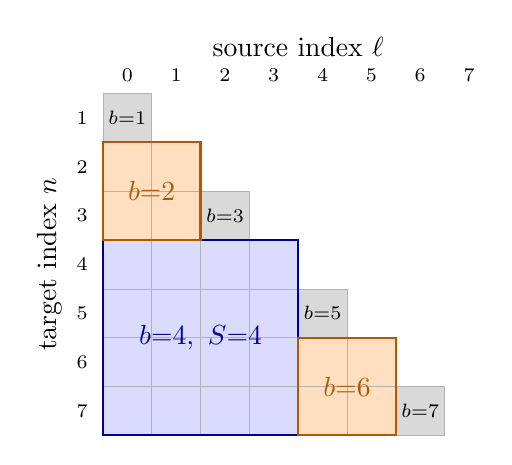
\begin{tikzpicture}[x=0.62cm, y=-0.62cm]
% shaded merge blocks
\fill[blue!14]   (0,4) rectangle (4,8);   % b=4, S=4
\fill[orange!25] (0,2) rectangle (2,4);   % b=2, S=2
\fill[orange!25] (4,6) rectangle (6,8);   % b=6, S=2
\fill[black!15]  (0,1) rectangle (1,2);   % b=1
\fill[black!15]  (2,3) rectangle (3,4);   % b=3
\fill[black!15]  (4,5) rectangle (5,6);   % b=5
\fill[black!15]  (6,7) rectangle (7,8);   % b=7
% cell grid over the strict lower triangle
\foreach \n in {1,...,7} {
  \foreach \l in {0,...,7} {
    \ifnum\l<\n
      \draw[gray!60, very thin] (\l,\n) rectangle (\l+1,\n+1);
    \fi
  }
}
% block outlines
\draw[blue!60!black, thick]   (0,4) rectangle (4,8);
\draw[orange!70!black, thick] (0,2) rectangle (2,4);
\draw[orange!70!black, thick] (4,6) rectangle (6,8);
% labels
\node[blue!60!black]   at (2,6)     {$b{=}4,\ S{=}4$};
\node[orange!70!black] at (1,3)     {$b{=}2$};
\node[orange!70!black] at (5,7)     {$b{=}6$};
\node at (0.5,1.5) {\scriptsize$b{=}1$};
\node at (2.5,3.5) {\scriptsize$b{=}3$};
\node at (4.5,5.5) {\scriptsize$b{=}5$};
\node at (6.5,7.5) {\scriptsize$b{=}7$};
% axes
\foreach \l in {0,...,7} { \node[above=1pt] at (\l+0.5,1) {\scriptsize$\l$}; }
\node[above=10pt] at (4,1) {source index $\ell$};
\foreach \n in {1,...,7} { \node[left=2pt] at (0,\n+0.5) {\scriptsize$\n$}; }
\node[rotate=90] at (-1.1,4.5) {target index $n$};
\end{tikzpicture}
\caption{The dependency triangle for $Q=8$, tiled by the merge schedule
of Section~\ref{sec:schedule}. Cell $(\ell,n)$ is the contribution of
source $u_\ell$ to target $G_n$. Each rectangle is one \emph{merge},
performed at boundary $b$ (after step $b-1$): sources $[\,b-S,\,b)$,
targets $[\,b,\,b+S)$, $S=2^{\vtwo(b)}$. The $4{\times}4$ block is
executed by FFT; small blocks below the cutoff run directly. Every cell
lies in exactly one rectangle (Theorem~\ref{thm:cover}).}
\label{fig:triangle}
\end{figure}

Figure~\ref{fig:triangle} shows the tiling for $Q=8$. Near the diagonal
the sequential constraint forces small batches (a target one step after
a source leaves no room); far from the diagonal, blocks of size
comparable to their distance from the diagonal fit comfortably. The
doubling pattern makes this precise: blocks of size $S=2^k$ sit at
distance $\sim 2^k$ from the diagonal, and each of the $\log_2 Q$ size
classes tiles an $O(Q)$-area band of the triangle.

\subsection{The merge schedule, and its correctness}
\label{sec:schedule}

Write $\vtwo(b)$ for the 2-adic valuation of the integer $b\ge1$: the
exponent of the largest power of two dividing $b$ (so $\vtwo(12)=2$,
$\vtwo(7)=0$; in code, $2^{\vtwo(b)} = b \mathbin{\&} (-b)$).

\medskip
\noindent\textbf{Schedule.} Immediately after step $n$ produces $u_n$,
let $b=n+1$. If $b<Q$, perform \emph{one} merge: with
$S = 2^{\vtwo(b)}$ and $E = \min(b+S,\,Q)$, add to the accumulators
\begin{equation}
G_{n'} \;\mathrel{+}=\; \sum_{\ell=b-S}^{b-1} B_{n'-\ell}\,u_\ell,
\qquad n' \in [\,b,\ E\,).
\label{eq:merge}
\end{equation}
When step $n'$ is later reached, its accumulator already equals the
full history $G_{n'}$ and is consumed with no further summation.

\medskip
The schedule is legal --- all sources in \eqref{eq:merge} exist at
boundary $b$, all targets lie in the future --- and it is
\emph{complete and non-redundant}:

\begin{lemma}[unique maximal valuation]
\label{lem:val}
Every nonempty integer interval $(\ell, n]$ contains exactly one
element of maximal 2-adic valuation.
\end{lemma}
\begin{proof}
Suppose $b_1<b_2$ in $(\ell,n]$ both have valuation exactly $v$. Their
difference is a positive multiple of $2^v$; it cannot equal $2^v$ (then
$b_2=b_1+2^v$ would have valuation $\ge v+1$), so $b_2-b_1\ge 2^{v+1}$
and the midpoint $b_1+2^v\in(b_1,b_2)\subset(\ell,n]$ has valuation
$\ge v+1$. Hence the maximal valuation in $(\ell,n]$ cannot be attained
twice: an element of strictly larger valuation would lie between the
two witnesses, contradicting maximality.
\end{proof}

\begin{theorem}[exactly-once covering]
\label{thm:cover}
For every pair $0\le\ell<n<Q$ there is exactly one boundary
$b\in(\ell,n]$ whose merge \eqref{eq:merge} transports $u_\ell$ to
$G_n$; namely the unique $b^*\in(\ell,n]$ of maximal valuation.
\end{theorem}
\begin{proof}
A boundary $b$ with $S=2^{\vtwo(b)}$ covers the pair iff
$b-S\le\ell<b\le n<b+S$.

\emph{Existence.} Let $b^*$ be the maximal-valuation element of
$(\ell,n]$ (Lemma~\ref{lem:val}), $v=\vtwo(b^*)$, $S^*=2^{v}$. Write
$b^*=S^*(2k+1)$. If $k=0$ then $b^*-S^*=0\le\ell$ trivially; if $k>0$
then $b^*-S^* = 2S^*k$ has valuation $\ge v+1$, so it cannot lie in
$(\ell,n]$, and since $b^*-S^*<b^*\le n$ this forces
$b^*-S^*\le\ell$. Likewise $b^*+S^*=2S^*(k+1)$ has valuation $\ge v+1$,
so $b^*+S^*\notin(\ell,n]$; since $b^*+S^*>\ell$ this forces
$b^*+S^*>n$. Thus $b^*$ covers the pair.

\emph{Uniqueness.} Suppose $b'\in(\ell,n]$ with $S'=2^{\vtwo(b')}$ also
covers the pair, $b'\ne b^*$. Then $\vtwo(b')<\vtwo(b^*)$, so $b^*$ is
a multiple of $2S'$. But the covering conditions place all of
$(\ell,n]\ni b^*$ inside the open interval $(b'-S',\,b'+S')$, whose
only multiples of $2S'$ are its excluded endpoints (writing
$b'=S'(2k'+1)$: $b'-S'=2S'k'$ and $b'+S'=2S'(k'+1)$ are
\emph{consecutive} multiples of $2S'$). Contradiction.
\end{proof}

\subsection{Executing a merge}
\label{sec:execute}

\paragraph{Small merges: direct.} Below a cutoff ($S<32$ in our
implementation) the merge runs as $S\times(E-b)$ block mat--vecs,
exactly like direct accumulation restricted to the rectangle. Over a
whole run these small merges touch each pair at most once, so their
total cost is bounded by the number of pairs within distance
$\mathrm{cutoff}$ of the diagonal: $O(Q\cdot\mathrm{cutoff})$ block
operations --- negligible, and it spares tiny FFTs whose overhead
exceeds their savings.

\paragraph{Large merges: FFT convolution.} Fix a merge $(b,S,E)$ and a
component pair: target row $a$, source column $c$ of the blocks. Define
length-$L$ arrays with $L=2S$:
\[
x[u] = u_{b-S+u}[c]\quad (0\le u<S,\ \text{zero-padded to } L),
\qquad
\beta[v] = B_v[a,c]\quad (1\le v\le 2S-1),\ \ \beta[0]=0,
\]
where lags $v\ge Q$ --- possible only when targets were clipped
($E<b+S$) --- are zero-filled. For $0\le w<E-b$ the needed sums are a
slice of the \emph{linear} convolution:
\[
\sum_{\ell=b-S}^{b-1} B_{(b+w)-\ell}[a,c]\;u_\ell[c]
= \sum_{u=0}^{S-1}\beta[S+w-u]\,x[u]
= (x*\beta)[\,S+w\,].
\]

\begin{lemma}[wrap-free window]
\label{lem:wrap}
The circular (FFT) convolution of length $L=2S$ agrees with the linear
convolution at positions $t\in[S,\,2S-1]$.
\end{lemma}
\begin{proof}
The linear convolution of supports $[0,S{-}1]$ and $[0,2S{-}1]$ has
support $[0,3S{-}2]$. Circular aliasing folds index $t+2S$ onto index
$t$; since $t+2S\le 3S-2$ forces $t\le S-2 < S$, no aliased mass lands
in $[S,2S-1]$.
\end{proof}

So the merge is: one forward FFT per source column ($s_{\dim}$ of
them), one forward FFT per component pair's lag segment
($t_{\dim}s_{\dim}$), pointwise multiply--accumulate into per-row
frequency accumulators, and one inverse FFT per target row
($t_{\dim}$); then add the real parts at positions $S..S+(E-b)-1$ into
the accumulators. All lengths are $2S$ with $S$ a power of two, so a
plain iterative radix-2 complex FFT \cite{ct1965} suffices --- about
sixty lines: bit-reversal permutation followed by butterfly passes,
split real/imaginary arrays, inverse transform leaving the $1/L$
scaling to the caller. Scratch buffers are grown on demand and reused
across merges.

\begin{remark}[caching variant]
The lag-segment transforms depend only on $(S,a,c)$, not on $b$, so
they could be computed once per size class and cached ($O(Q\log Q)$
extra memory). We recompute them lazily per merge --- simpler, $O(1)$
extra memory, and measured to be cheap.
\end{remark}

\subsection{Operation count}
\label{sec:complexity}

\emph{Merge census.} Boundaries with $\vtwo(b)=k$ are
$b = 2^k(2j+1) < Q$, i.e.\ about $Q/2^{k+1}$ merges of size $S=2^k$,
for $k = 0,1,\dots,\lfloor\log_2 Q\rfloor$. (Sanity check via areas:
size-$2^k$ merges cover $(Q/2^{k+1})\cdot 4^k = Q\,2^{k-1}$ pairs;
summing over $k$ gives $\sum_k Q\,2^{k-1}\approx Q^2/2$, the whole
triangle, consistent with Theorem~\ref{thm:cover}.)

\emph{Cost per merge.} With $D=\max(t_{\dim},s_{\dim})$: $O(D^2)$ FFTs
of length $2S$ at $O(S\log S)$ each, plus $O(D^2 S)$ pointwise work
--- $O(D^2\,S\log S)$ total.

\emph{Total.}
\[
\sum_{k=0}^{\log_2 Q} \underbrace{\frac{Q}{2^{k+1}}}_{\#\text{merges}}
\cdot O\!\bigl(D^2\, 2^k\, k\bigr)
\;=\; O\!\Bigl(D^2\, Q \sum_{k=0}^{\log_2 Q} k\Bigr)
\;=\; O\!\bigl(D^2\, Q\log^2 Q\bigr).
\]
An equivalent way to see the $\log^2$: each source vector participates
in at most one merge per size class (about $\log_2 Q$ merges over its
lifetime --- in Figure~\ref{fig:triangle}, each column meets one
rectangle of each size), and inside a size-$2^k$ merge its per-element
FFT share is $O(k)$; summing $O(k)$ over $k\le\log_2 Q$ gives
$O(\log^2 Q)$ work per source, versus $O(Q)$ for direct accumulation
and $O(\log Q)$ for a single offline FFT. The one extra log factor is
the price of sequentiality.

\emph{Memory.} The lag-block table ($Q\,t_{\dim}s_{\dim}$ doubles ---
1.3\,MB for a scalar $p=3$ run with $Q\approx18{,}000$), the
accumulators and stored sources ($Q(t_{\dim}{+}s_{\dim})$), and
$O(D^2 S_{\max})$ scratch: $O(D^2 Q)$ overall.

\emph{Empirical confirmation.} After the change, measured times double
(rather than quadruple) per doubling of $N$: 0.05\,s, 0.26\,s, 1.32\,s
at $N = 40$k, 160k, 640k (Section~\ref{sec:results}) --- the residual
super-linearity being the $\log^2$ factor plus the $O(Q)$ local solves.

\subsection{Why we implemented this, rather than something else}
\label{sec:why}

\begin{itemize}
\item \textbf{The quadratic wall is the binding constraint.} At the
  resolutions our applications need ($N\sim10^5$--$10^6$ samples;
  long-time electrochemical transients), $O(Q^2)$ costs minutes and
  each refinement quadruples it. No constant-factor tuning
  (vectorization, cache blocking) changes that shape; only an
  asymptotically better summation does.
\item \textbf{It is an evaluation strategy, not a new method.} Because
  the algorithm computes the same sums reordered
  (take-home~5), it drops into each existing driver by replacing
  ``form $G_n$ by a loop'' with ``read accumulator; after the step,
  push $u_n$'' --- no change to discretization, step maps, boundary
  handling, or public API, and the entire existing test suite remains
  the oracle. Alternatives (fast-oblivious quadrature
  \cite{schadle2006}, kernel compression) change the representation of
  the history and would have been a rewrite, not a retrofit.
\item \textbf{It composes with every solver family at once.} One
  engine (Section~\ref{sec:engine}) serves VIE-1 (both variants),
  VIE-2 and VIDE, scalar through $d$-component systems, because they
  differ only in their lag-block tables and source vectors.
\item \textbf{Its floating-point behaviour is controllable.} Sum
  reordering and FFT rounding perturb results at the
  $\varepsilon\log Q$ level --- quantifiable, verifiable, and (unlike
  approximation-based accelerations) carrying no method-error budget
  to tune. This mattered under the reproducibility policy of
  Section~\ref{sec:fp}.
\end{itemize}

%=====================================================================
\section{Application to the \voles{} sampled-data solvers}
\label{sec:apply}

\subsection{The lag blocks of each solver family}
\label{sec:blocks}

It remains to exhibit each family's history in the form
\eqref{eq:online}. In all cases the mesh-interval width is
$\Delta=c^2h$ and $w_j$ denotes the interpolatory quadrature weights of
the node set $\{c_j/c\}$.

\paragraph{VIE-1 and VIE-2.} The scalar blocks are pure kernel samples
(systems replace each entry by the corresponding $d\times d$ kernel
block):
\begin{equation}
B_v[i,j] \;=\; w_j\,
K\!\bigl(\,[\,v\,c^2 + (c_i-c_j)\,c\,]\,h\,\bigr),
\qquad i,j=1,\dots,m,\quad v = n-\ell,
\label{eq:BNL}
\end{equation}
entering the right-hand side as $\pm\Delta\sum_{\ell<n}B_{n-\ell}U_\ell$
(sign per family). We fold the prefactor into the stored table,
$\widetilde B_v = \Delta B_v$, once at initialization. The continuous
(``force-continuous'') VIE-1 variant differs from the discontinuous one
only in local terms (a boundary value propagated interval to interval);
its history is the same $B_v$ and needs no special treatment.

\paragraph{VIDE.} The history couples to both the collocation values
$Y_\ell$ of $y'$ and the propagated boundary values
$y^{\mathrm{bnd}}_\ell=y(t_\ell)$:
\begin{equation}
G_n \;=\; \sum_{\ell<n}\Bigl[\;\Delta^2\, C_{n-\ell}\,Y_\ell
 \;+\; \Delta\, \kappa_{n-\ell}\, y^{\mathrm{bnd}}_\ell\;\Bigr],
\label{eq:vide-history}
\end{equation}
where the matrix $C_v$ and vector $\kappa_v$ are fixed contractions of
kernel samples at indices $v c^2 + (c_i-c_k)c$ against precomputed node
tensors (their exact formulas are the existing solver's and are not
modified). This fits \eqref{eq:online} with a \emph{rectangular}
augmented block: source vector $s_\ell = [\,Y_\ell;\
y^{\mathrm{bnd}}_\ell\,]$ of dimension $s_{\dim}=dm+d$ and lag block
$\widetilde B_v = [\,\Delta^2 C_v \;|\; \Delta\,\kappa_v\,]$ of shape
$dm\times(dm+d)$. One subtlety: push the boundary value \emph{at the
start} of interval $\ell$ (that is what \eqref{eq:vide-history} uses),
even though the push happens after the interval solve, by which time
the end value has also been computed.

\subsection{The history engine}
\label{sec:engine}

Package Sections~\ref{sec:schedule}--\ref{sec:execute} as a
self-contained object with runtime dimensions
$(t_{\dim}, s_{\dim})$ and three operations:
\begin{description}
\item[\texttt{initialize}$(Q, t_{\dim}, s_{\dim})$:] allocate the lag
  table (length $Q\,t_{\dim}s_{\dim}$, filled by the caller with all
  scalings folded in; lag 0 unused), the accumulator array
  ($Q\times t_{\dim}$, zeroed), and the source store
  ($Q\times s_{\dim}$).
\item[\texttt{G}$(n)$:] return accumulator row $n$ (valid once sources
  $0..n{-}1$ are pushed).
\item[\texttt{push}$(s)$:] store $s$ as the next source; with
  $b=(\text{count})$, $S=b\,\&\,(-b)$, $E=\min(b+S,Q)$, run the single
  merge of \eqref{eq:merge} --- direct if $S<32$, else the FFT form of
  Section~\ref{sec:execute}.
\end{description}
Driver changes are then minimal and identical across families:
\begin{center}
\emph{replace} ``\,$G\gets$ loop over $\ell<n$\,'' \emph{by}
``\,$G\gets\texttt{G}(n)$\,''; \quad
\emph{append} ``\,\texttt{push}$(u_n)$\,'' after each interval solve.
\end{center}
We wired it into all six compiled drivers (VIE-1 discontinuous and
continuous, VIE-2, VIDE; scalar and system variants) and, because in
our applications systems with more than eight components are common,
also into the runtime-dimension drivers used for $d>8$ (where the local
solves go through LAPACK). The compile-time drivers use a thin
fixed-dimension wrapper over the same runtime-dimension core --- a
refactor verified to change no output bit.

%=====================================================================
\section{The companion optimization: one-row weight assembly in
function mode}
\label{sec:assembly}

The function-mode solvers spend their time not in stepping but in
\emph{building} their weight tensor
\begin{equation}
W[n,i,l,k] \;=\;
\int_{t_l}^{t_{l+1}} K\bigl(\tau_{n,i}-s\bigr)\,
L_k\!\Bigl(\tfrac{s-t_l}{h_l}\Bigr)\dd s ,
\qquad l < n,
\label{eq:Wdef}
\end{equation}
($L_k$: reference-interval basis polynomials; plus \emph{diagonal}
blocks $l=n$ with upper limit $\tau_{n,i}$), evaluated by numerical
quadrature per block --- $O(M^2)$ quadratures in all. On a uniform mesh
the substitution $\sigma=s-t_l$ gives
\begin{equation}
W[n,i,l,k] \;=\;
\int_{0}^{h} K\bigl((n-l)h + x_i h - \sigma\bigr)\,
L_k(\sigma/h)\dd\sigma ,
\label{eq:Wshift}
\end{equation}
a function of the lag $n-l$ alone; the diagonal blocks are independent
of $n$ altogether. This holds for weakly singular kernels too, provided
the declared singularity is convolution-style (locations in $u=t-s$):
the singular point falls at the same lag-relative position in every
row, so even the classification of blocks as smooth or singular is
lag-invariant.

\subsection{The existing quadrature machinery}
Reproducing the optimization requires knowing how a block is evaluated:
\begin{enumerate}
\item \textbf{Classification.} Declared singular $s$-locations for
  $\tau_{n,i}$ are tested against $[a,b]=[t_l,t_{l+1}]$ with tolerance
  $10^{-12}\max(1,b-a)$; interior or endpoint hits send the block to
  the adaptive path.
\item \textbf{Smooth path.} Fixed-order Gauss--Legendre at two orders
  (6 and 8), all basis functions at once; basis entry $k$ is
  \emph{accepted} iff $|v_1-v_2|\le 10^{-9}\max(1,|v_2|)$, storing the
  order-8 value; rejected entries fall back per-entry to the adaptive
  path.
\item \textbf{Adaptive path.} \texttt{scipy.integrate.quad} (QUADPACK
  \cite{quadpack}), subdivision limit 100, \texttt{points=} hints for
  interior singularities.
\end{enumerate}

\subsection{The algorithm}
Equation \eqref{eq:Wshift} suggests integrating a single row that
contains every lag --- row $M{-}1$ --- and copying blocks
band-diagonally, $W[n,:,l]\leftarrow W[M{-}1,:,\,l+(M{-}1{-}n)]$, with
the diagonal template likewise. Our implementation does exactly this
for blocks whose row-$(M{-}1)$ evaluation came entirely from the
\emph{deterministic} fixed-order GL path, and \emph{re-evaluates
per row}, with byte-identical calls, every block that involved adaptive
quadrature (singularity-classified blocks and two-order-check
fallbacks). The reason for treating the two classes differently is a
floating-point reproducibility requirement, discussed in
Section~\ref{sec:fp}; here we record the algorithm:

\begin{algorithm}[t]
\caption{Uniform-mesh weight-tensor assembly}
\label{alg:assembly}
\begin{algorithmic}[1]
\State detect uniformity ($\max_l h_l-\min_l h_l\le10^{-12}\bar h$) and
  convolution-style singularity declaration; else run the general
  $O(M^2)$ loop unchanged
\State integrate row $M{-}1$ with the unchanged per-block machinery,
  recording masks $\mathrm{ok}_{\mathrm{off}}[i,\mu]$ (off-diagonal
  block at lag $\mu$, node $i$ fully GL-accepted) and
  $\mathrm{ok}_{\mathrm{diag}}[i]$
\State copy row $M{-}1$ band-diagonally into every row (one contiguous
  slice per row); copy the diagonal template
\State $\mathrm{cleanlag}[\mu]\gets\bigwedge_i\mathrm{ok}_{\mathrm{off}}[i,\mu]$
\For{$n=0,\dots,M-2$}
  \State work list $\{\,l=n-\mu:\ \mu\in[1,n],\ \neg\mathrm{cleanlag}[\mu]\,\}$
    (one \texttt{nonzero}, not an $O(n)$ scan)
  \State for each listed block and each node $i$ with
    $\neg\mathrm{ok}_{\mathrm{off}}[i,n-l]$: re-run classification, GL +
    two-order check, and fallbacks exactly as the general path would;
    overwrite
  \State likewise re-run the diagonal block for each $i$ with
    $\neg\mathrm{ok}_{\mathrm{diag}}[i]$
\EndFor
\end{algorithmic}
\end{algorithm}

Two implementation notes. (i)~\emph{Subset determinism}: when only a
subset of a block's nodes is recomputed, the vectorized GL evaluation
over the subset must reproduce, per node, the full-set values bit for
bit; this holds because the per-node arithmetic (kernel samples per
node--abscissa pair, contraction per node) is independent, as in the
existing \texttt{einsum} formulation. (ii)~\emph{Cost}: $O(M)$
quadratures for the integrated row, plus per-row repairs --- for an
Abel kernel the $p$ diagonal blocks and a few near-diagonal fallback
lags per row, still $O(M)$ in total --- plus $O(M^2p^2)$ pure memory
copies. Smooth kernels, having no adaptive blocks, gain the most
(measured $\sim$80$\times$ at $M=320$); Abel kernels gain
3--26$\times$ and now scale linearly. Non-uniform (graded) meshes and
callable singularity locators take the untouched general path,
verified bit-identical.

%=====================================================================
\section{Floating-point reproducibility policy}
\label{sec:fp}

The acceptance criterion for this work, fixed during review of an
early draft of the assembly optimization, was: \emph{optimized code
must agree with the original to numerical precision} --- rounding-level
deviations are acceptable, tolerance-level deviations are not. Three
classes of deviation arise:

\begin{enumerate}
\item \textbf{Reuse of deterministic quadrature (permitted).}
  Fixed-order GL is a pure function of interval endpoints and integrand
  samples. Evaluating an equal-lag block at a shifted absolute position
  perturbs each abscissa and each $\tau-s$ argument by a few ulps of
  the absolute times; equal-lag GL values agree to $\sim10^{-15}$
  relative. Copying them is as good as recomputing.
\item \textbf{Reuse of adaptive quadrature (forbidden).} QUADPACK's
  subdivision and extrapolation decisions branch on error estimates
  formed from absolute coordinates, and its result is guaranteed only
  to its own tolerance ($\approx1.5\times10^{-8}$). Empirically,
  equal-lag adaptive blocks evaluated in different rows differ by
  $10^{-10}$--$10^{-9}$ --- \emph{including in the original code},
  which silently assigns slightly different values to mathematically
  identical blocks. Reusing one row's value stays within that
  pre-existing scatter but is not rounding-level identical to the
  per-row result; under the criterion we therefore recompute all
  adaptive blocks per row (making them bit-identical), at the price of
  keeping an $O(M)$ per-row quadrature cost on singular kernels. The
  rejected ``full reuse'' variant is a further $\sim$8$\times$ on Abel
  kernels and is worth revisiting if the criterion is ever relaxed. A
  residual measure-zero caveat: a two-order acceptance check comparing
  values that differ across rows by $10^{-15}$ against a sharp
  threshold could in principle flip for some row; the consequence is
  bounded by the GL-versus-adaptive gap ($\lesssim10^{-9}$) on that
  single block.
\item \textbf{Summation restructuring (permitted).} The history engine
  reorders additions and routes some through FFTs. Deviations are
  rounding-level, $O(\varepsilon\log Q)$ relative to the magnitudes in
  the sums, mildly amplified by problem conditioning (first-kind
  equations show the largest values) --- the same class as compiling
  with different SIMD settings, and unavoidable in \emph{any} fast
  summation. Measured worst case over the entire verification battery:
  $2\times10^{-11}$ of solution scale; typical
  $10^{-15}$--$10^{-13}$.
\end{enumerate}

%=====================================================================
\section{Verification methodology}
\label{sec:verification}

Reproducing the verification matters as much as the algorithms.

\paragraph{A/B protocol.} Build the unmodified reference and the
optimized branch as two installations; run \emph{identical} scripts
against both; compare saved outputs. The certificate sought is
agreement with the old code, not correctness of the discretization ---
the latter is the existing test suite's job (all 363 tests pass on the
optimized build, $1.8\times$ faster).

\paragraph{Coverage.} (i)~Every problem spec of the repository test
suite (20 specs across the three families, including the weakly
singular ones), each run through both the sampled and function
solvers; (ii)~each at the suite's own size \emph{and} at a larger size
that actually exercises the FFT merges and the one-row assembly (the
suite's $Q=10$ never reaches the merge cutoff); (iii)~vector cases
($d=2$) and a $d=10$ battery for the runtime-dimension drivers ---
about 100 A/B cases in all.

\paragraph{Two traps, so the reader avoids them.}
\begin{enumerate}
\item \textbf{Growing-resolvent problems.} Enlarging a test problem by
  extending its horizon at fixed step is wrong. Several suite problems
  have exponentially growing resolvents (a second-kind equation with
  $K=2$ grows like $e^{2t}$); by $T\approx46$ the numerical solution in
  \emph{both} builds is dominated by rounding-seeded growing modes
  ($10^{6}$--$10^{24}$ against true solutions of $O(1)$--$O(10^3)$),
  and the two builds then differ at $O(1)$ relative --- chaotic
  amplification of last-bit noise, not a bug. Keep the horizon; refine
  the step to reach large $Q$. After this correction the worst case
  dropped from $O(1)$ to $2\times10^{-11}$.
\item \textbf{Zero crossings.} Element-wise relative comparison fails
  spuriously where solutions cross zero: rounding noise has absolute
  size set by the magnitudes in the \emph{computation} (history sums
  involve the whole solution), not by the local output value. Use a
  per-problem scale-aware floor,
  $\texttt{atol}=\mathrm{tol}\cdot\max|y|$: with
  $\mathrm{rtol}=\mathrm{tol}=10^{-10}$ all finite cases pass; with
  \texttt{numpy} defaults all 100 cases pass.
\end{enumerate}
Two deliberately borderline extra cases (continuous VIE-1 with nodes
$\{0.5,1.0\}$, amplification exactly $\rho=1$) overflow to
\texttt{inf}/NaN on long runs --- identically in both builds (same
positions, finite prefixes agreeing to $\sim10^{-167}$ relative); they
are excluded from finite statistics.

\paragraph{Bitwise identities.} Verified exactly: (a)~graded
(non-uniform) meshes produce bit-identical weight tensors (the fast
path must not engage); (b)~the runtime-dimension refactor of the
history engine changed no output bit over the whole battery.

\paragraph{Recommended test order for a reimplementation.}
(a)~history engine versus direct summation on \emph{random} lag tables
--- a pure unit test with no solver attached; (b)~the A/B battery
above; (c)~the full existing test suite; (d)~timing curves ---
confirm $4\times$ per doubling becomes $\approx2\times$.

%=====================================================================
\section{Measured results}
\label{sec:results}

Apple-silicon laptop, July 2026; collocation order $p=3$
(\texttt{coll\_divs}=3, \texttt{coll\_choices}=[1,2,3]) unless noted;
``old'' is upstream \texttt{main} built identically (extrapolated
entries marked).

\begin{center}
\begin{tabular}{lllll}
\toprule
case & old & new & speedup & scaling change\\
\midrule
sampled VIE-1, $N=160{,}001$ & 19.9\,s & 0.26\,s & 77$\times$ &
  $O(Q^2)\to O(Q\log^2 Q)$\\
sampled VIE-1, $N=640{,}001$ & $\sim$320\,s & 1.32\,s & $\sim$240$\times$ & \\
sampled VIE-2, $d=10$, $N=36{,}001$ & 79.9\,s & 2.56\,s & 31$\times$ &
  runtime-$d$ drivers\\
function, smooth kernel, $M=320$ & 1.02\,s & 0.013\,s & $\sim$80$\times$ &
  $O(M^2)\to O(M)$ quads\\
function, Abel kernel, $M=320$ & 3.31\,s & 0.98\,s & 3.4$\times$ & \\
function, Abel, $M=2560$ & $\sim$210\,s & 8.0\,s & $\sim$26$\times$ & \\
repository test suite (363 tests) & 35.5\,s & 19.4\,s & 1.8$\times$ & \\
\bottomrule
\end{tabular}
\end{center}

Per-test suite timings and full difference distributions are in the
companion figures (\texttt{plot\_speedups.png},
\texttt{plot\_differences.png}).

\subsection*{Known limitations / next steps}
Graded (non-uniform) meshes take the original paths by design; the
natural extension is a graded-start/uniform-tail hybrid. The
function-mode dense weight tensor still costs $O(M^2p^2)$ memory; a
lag-indexed stepping entry point would cut it to $O(Mp^2)$. Function
mode has no $d>8$ capability at all (it errors rather than falling
back); given that large systems matter in our applications, that is a
missing feature, not a slow path. And the ``full reuse'' assembly
variant of Section~\ref{sec:fp} remains available should the
reproducibility criterion ever be relaxed.

\begin{thebibliography}{9}

\bibitem{hls1985}
E. Hairer, C. Lubich, and M. Schlichte,
\emph{Fast numerical solution of nonlinear Volterra convolution
equations}, SIAM J. Sci. Stat. Comput. \textbf{6} (1985) 532--541.

\bibitem{schadle2006}
A. Sch\"adle, M. L\'opez-Fern\'andez, and C. Lubich,
\emph{Fast and oblivious convolution quadrature},
SIAM J. Sci. Comput. \textbf{28} (2006) 421--438.

\bibitem{vdh2002}
J. van der Hoeven, \emph{Relax, but don't be too lazy},
J. Symbolic Comput. \textbf{34} (2002) 479--542.

\bibitem{ct1965}
J. W. Cooley and J. W. Tukey, \emph{An algorithm for the machine
calculation of complex Fourier series},
Math. Comp. \textbf{19} (1965) 297--301.

\bibitem{brunner2004}
H. Brunner, \emph{Collocation Methods for Volterra Integral and Related
Functional Differential Equations}, Cambridge University Press, 2004.

\bibitem{olmstead1968}
M. L. Olmstead and R. S. Nicholson,
\emph{A method based on polynomial approximations for numerical solution
of Volterra integral equations},
J. Electroanal. Chem. \textbf{16} (1968) 145--151.

\bibitem{quadpack}
R. Piessens, E. de Doncker-Kapenga, C. \"Uberhuber, and D. Kahaner,
\emph{QUADPACK: A Subroutine Package for Automatic Integration},
Springer, 1983.

\end{thebibliography}

\end{document}
